\documentclass[12pt]{article}
\usepackage[utf8]{inputenc}
\usepackage[T1]{fontenc}
\usepackage{amsmath,amsfonts,amssymb}
\usepackage{graphicx}
\usepackage{a4wide}
\usepackage[citestyle=numeric,style=numeric,backend=bibtex,sorting=none]{biblatex}
\renewcommand{\baselinestretch}{1.36}

\usepackage{doi}
\usepackage{makecell}
\usepackage{subfig}
\addbibresource{references.bib}


\title{Correlation-based Algorithm for pointwise predicting the value of a multivariate time series}

\author{%
	Maxim Divilkovskiy\footnote{Forecsys, mdivilkovskij@gmail.com},  %
	Konstantin Yakovlev\footnote{Forecsys,  bicst808@gmail.com},  %
	Vadim Strijov\footnote{Forecsys,  strijov@gmail.com},  %
}
%\date{}
\hypersetup{pdfauthor={Maxim Divilkovskiy},}
\graphicspath{ {./figures/} }% Remove. Put the figures in \.

\begin{document}
\maketitle

\begin{abstract}
The paper investigates a time series prediction problem. It constructs a pointwise prediction model for a set of time series. These time series have high variance and high covariance. Paper introduces space of pairwise distances between time series and analyses its properties. In this space, the pairwise distance matrix is predicted in its dynamics. The time series values are reconstructed at the next time moment with this matrix. The authors propose several methods for the pointwise prediction of time series space using the reconstruction reconstructed space of the pairwise distance matrices. We prove the existence of multiple time series values satisfying the same pairwise distance matrix. It presents two algorithms based on the use of matrices constructed over different time intervals using pairwise correlation. The paper derives an explicit view of the reconstructed values through the pairwise correlation matrix. Also, it derives an evaluation of the quality of the reconstruction when noise is added to the pairwise distance matrices. The novelty of the method is that the prediction is not done in the original space but in the space of pairwise distances.


\end{abstract}

\textbf{Keywords:} Metric Non-Convex Optimization, Time Series Forecasting, Singular Value Decomposition, Pearson Correlation Coefficient

\section{Introduction}
 	In this research the authors present a new method for pointwise time series prediction. Time series have high pairwise covariance and high variance. Pointwise prediction consists of calculating the values of the time series at the next point in time using the available historical data for the previous several points in time. A set of $d$ time series, each of which consists of $t$ time moments forms a multivariate time series. We call the multivariate time series space isomorphic to $\mathbb{R}^{d \times t}$ the source time series space. The prediction problem divides into three stages. First, transform the source space of the time series into a metric space by constructing a matrix of pairwise distances. Second, do the prediction of the pairwise distances matrix at the next moment of time in the metric space. Third, use the predicted matrix to reconstruct the result into the source space. In the theoretical part of the paper, we prove the necessity of predicting at least two matrices. We show that the uniqueness of the reconstructed result in the source space requires the use of several matrices corresponding to different time intervals. We focus mostly on the last step. We present experiments for the case of accurate matrix prediction and for the matrix prediction with the addition of normal noise to the values.

	Existing time series prediction methods such as LSTM \cite{LSTM}, SSA \cite{SSA} and other \cite{Biosignals, boyd2017multiperiod} predict the value of a univariate series. These methods can be modified to predict also a set of time series. For this purpose, it is sufficient to present a set of series as one multivariate series. This approach does not explicitly model the dependencies between different series. In contrast, we propose to analyze the change in \emph{set} of time series. Our approach explicitly uses the relationships between them as information. A similar study is carried out in the \cite{MulticorrelatedQuadratic} paper, but it emphasizes on the feature selection problem. It consists in selecting such a subset of the original time series for which it is possible to make a predict of sufficient quality.
	
	Recent studies \cite{haoyietal-informer-2021,haoyietal-informerEx-2023,wu2021autoformer,liu2022pyraformer} use popular transformer-based models. Transformer models were originally proposed for natural language processing problems, such as translation and text-completion \cite{NIPS2017_3f5ee243}. However, since many language problems deal with text as a sequence in time, the same approaches may be used for time series predicting. The Crossformer model \cite{zhang2023crossformer} uses cross-dimensional dependency.  However, it does not explicitly model the distance function between time series.
	
	Further, we study conditions on the distance function between rows under which there is a way to reconstruct the values of the time series. We prove the insufficiency of one matrix to reconstruct the answer. We propose two methods for the value prediction using several matrices for the case of accurate prediction and for the case of prediction with non-zero noise. Also, we propose a reconstruction algorithm based on two theorems about the explicit formula of the result in time series space using pairwise correlation as a function of pairwise distance between rows. Mean Squared Error and Mean Absolute Error are used as quality criteria. It is shown in the article \cite{jadon2022comprehensive} that they are the most suitable for the task of time series prediction.
	
	In the experiments section we measure losses of our Algorithm on synthetic dataset and Electricity Transformer Temperature dataset. We show that as the count of matrices used increases, the loss decreases.

\section{Point-wise prediction of a set of time series}

The time series with $t$ moments in time is a set of $t$ elements:
\[
[\mathbf{x}_1, \mathbf{x}_2, \ldots, \mathbf{x}_t],\qquad \text{for each } k: \mathbf{x}_k \in \mathbb{R}^d,
\]
where $\mathbf{x}_{t_i, k} \in \mathbb{R}$ is the value of the series with index $k$ at the time moment $t_i$.
One has to predict $\mathbf{x}_{t+1}$, which is the value of time series at the time moment $t+1$. The matrix $\mathbf{x}$ of size $t \times d$ is treated as a \emph{multivariate} time series, treating the value at a point as an element of space $\mathbb{R}^d$.

Prediction errors are calculated with two functions,
\[
\text{MAE} = \frac{1}{d}{\sum_{i=1}^{d} |\mathbf{x}_{t+1} - \mathbf{\hat{x}}_{t+1}|}, 
\qquad \text{and} \qquad 
\text{MSE} = \frac{1}{d}{\sum_{i=1}^{d} (\mathbf{x}_{t+1} - \mathbf{\hat{x}}_{t+1})^2}.
\]

\section{Reconstruction of time series by a predicted distance matrix}

In this section we formulate general algorithm of reconstruction the time series values in the moment $t+1$ from information about time moments $1, 2, \ldots, t$. Novelty of out algorithm consists in usage of \emph{pairwise distance matrices}.

Construct distance matrices between a set of time series values according to the scheme below:
\begin{align*}
	[&\mathbf{x}_1, \ldots, \mathbf{x}_s] \rightarrow \mathbf{\Sigma}_s, \\
	[&\mathbf{x}_2, \ldots, \mathbf{x}_{s+1}] \rightarrow \mathbf{\Sigma}_{s+1}, \\
	&\vdots \\
	[&\mathbf{x}_{t-s}, \ldots, \mathbf{x}_t] \rightarrow \mathbf{\Sigma}_{t}.
\end{align*}
Each $\mathbf{\Sigma}_i$ is a matrix of pairwise distances of size $d \times d$. An element of the matrix $\mathbf{\Sigma}_{i,j}$ is the value of the distance between rows $i$ and $j$. We describe the construction formula as well as the choice of the distance function in the following sections.

Predict the matrix $\hat{\mathbf{\Sigma}}_{t+1}$ from matrices $\mathbf{\Sigma}_s, \mathbf{\Sigma}_{s+1} \ldots, \mathbf{\Sigma}_{t}$.

Find such $\mathbf{\hat{x}}_{t+1}$, that \[ ||\hat{\mathbf{\Sigma}}_{t+1} - \bar{\mathbf{\Sigma}}_{t+1}||_2^2 \rightarrow \min_{\mathbf{\hat{x}}_{t+1}}, \tag{\textasteriskcentered} \label{minimization}\] where $\bar{\mathbf{\Sigma}}_{t+1}$ is the distance matrix, constructed from the set $[\mathbf{x}_{t-s+1}, \ldots, \mathbf{x}_{t}, \mathbf{\hat{x}}_{t+1}]$. Achieving a minimum by this function would mean that $\hat{\mathbf{\Sigma}}_{t+1}$ are $\bar{\mathbf{\Sigma}}_{t+1}$ equal. In turn, this means that the found continuation of the series at time $t+1$ has a distance matrix equal to the prediction. In general, this function is \emph{non-convex} and there can be several minimums. We address this problem in the following sections.

\section{Existence of several values of a series satisfying same distance matrix}

The existence of several solutions to the minimization problem $\eqref{minimization}$ is the central problem we consider in this paper. In this section we show that using one matrix constructed by an arbitrary metric it is possible to reconstruct several different values of the series at the next moment of time. A solution to this problem in the case of using pairwise correlation as a function of distance between certain time series is proposed in the next section.

We now describe the reconstruction of the prediction from the matrix $\mathbf{\Sigma}_{t+1}$ to source time series space, where $\mathbf{\Sigma}_{t+1}$ is the matrix of pairwise distances corresponding to the multivariate series $\mathbf{x}=[\mathbf{x_1}, \ldots, \mathbf{x_{t+1}}]$.

Given a pairwise distance matrix $\mathbf{\Sigma}$ of size $d \times d$ for multivariate time series $\mathbf{x} \in \mathbb{R}^{d \times (t+1)}$. $\hat{\mathbf{x}}_{t+1} \in \mathbb{R}^d$ is predicted. Also, the metric \[ \rho : \mathbb{R}^{t+1} \times \mathbb{R}^{t+1} \rightarrow \mathbb{R}, \] defined on time series, satisfies the properties of the metric. Which are \[\mathbf{\Sigma}_{i,j} = \rho(\mathbf{x}_{1 \ldots t, i} \circ \hat{\mathbf{x}}_{t+1, i}, \mathbf{x}_{1 \ldots t, j} \circ \hat{\mathbf{x}}_{t+1, j}),\] where $\circ$ denotes the concatenation of vector with value.

One of the fundamental metrics for calculating distance of objects in $\mathbb{R^d}$ is the Euclidean metric. With this example, we show that there can be several reconstructions with the same distance matrices. In the case of the Euclidean metric, the number of answers is infinite, which we show below:
\[\mathbf{\Sigma}_{i,j} = \rho(\mathbf{x}_{1 \ldots t, i} \circ \hat{\mathbf{x}}_{t+1, i}, \mathbf{x}_{1 \ldots t, j} \circ \hat{\mathbf{x}}_{t+1, j})=\sqrt{\left(\sum_{k=1}^t (\mathbf{x}_{k,i}-\mathbf{x}_{k,j})^2\right) + (\hat{\mathbf{x}}_{t+1, i}-\hat{\mathbf{x}}_{t+1, j})^2}.\]

Using this metric results in the fact that adding some constant $C$ to all $\hat{\mathbf{x}}_{t+1, i}$ does not change the answer:
\begin{gather*}
	\sqrt{\left(\sum_{k=1}^t (\mathbf{x}_{k,i}-\mathbf{x}_{k,j})^2\right) + (\hat{\mathbf{x}}_{t+1, i}-\hat{\mathbf{x}}_{t+1, j})^2} =\\
	= \sqrt{\left(\sum_{k=1}^t (\mathbf{x}_{k,i}-\mathbf{x}_{k,j})^2\right) + [(\hat{\mathbf{x}}_{t+1, i} + C) -(\hat{\mathbf{x}}_{t+1, j} + C)]^2}.
\end{gather*}

In the case of the time series prediction problem, this property is critical because even if the matrix $\mathbf{\Sigma}$ is predicted accurately, there are infinitely many time series values at time $t+1$ corresponding to this matrix. See Figure \ref{fig:fig1} for the example of this effect.
\begin{figure}[!htbp]
	\centering
	\subfloat[Reference functions]{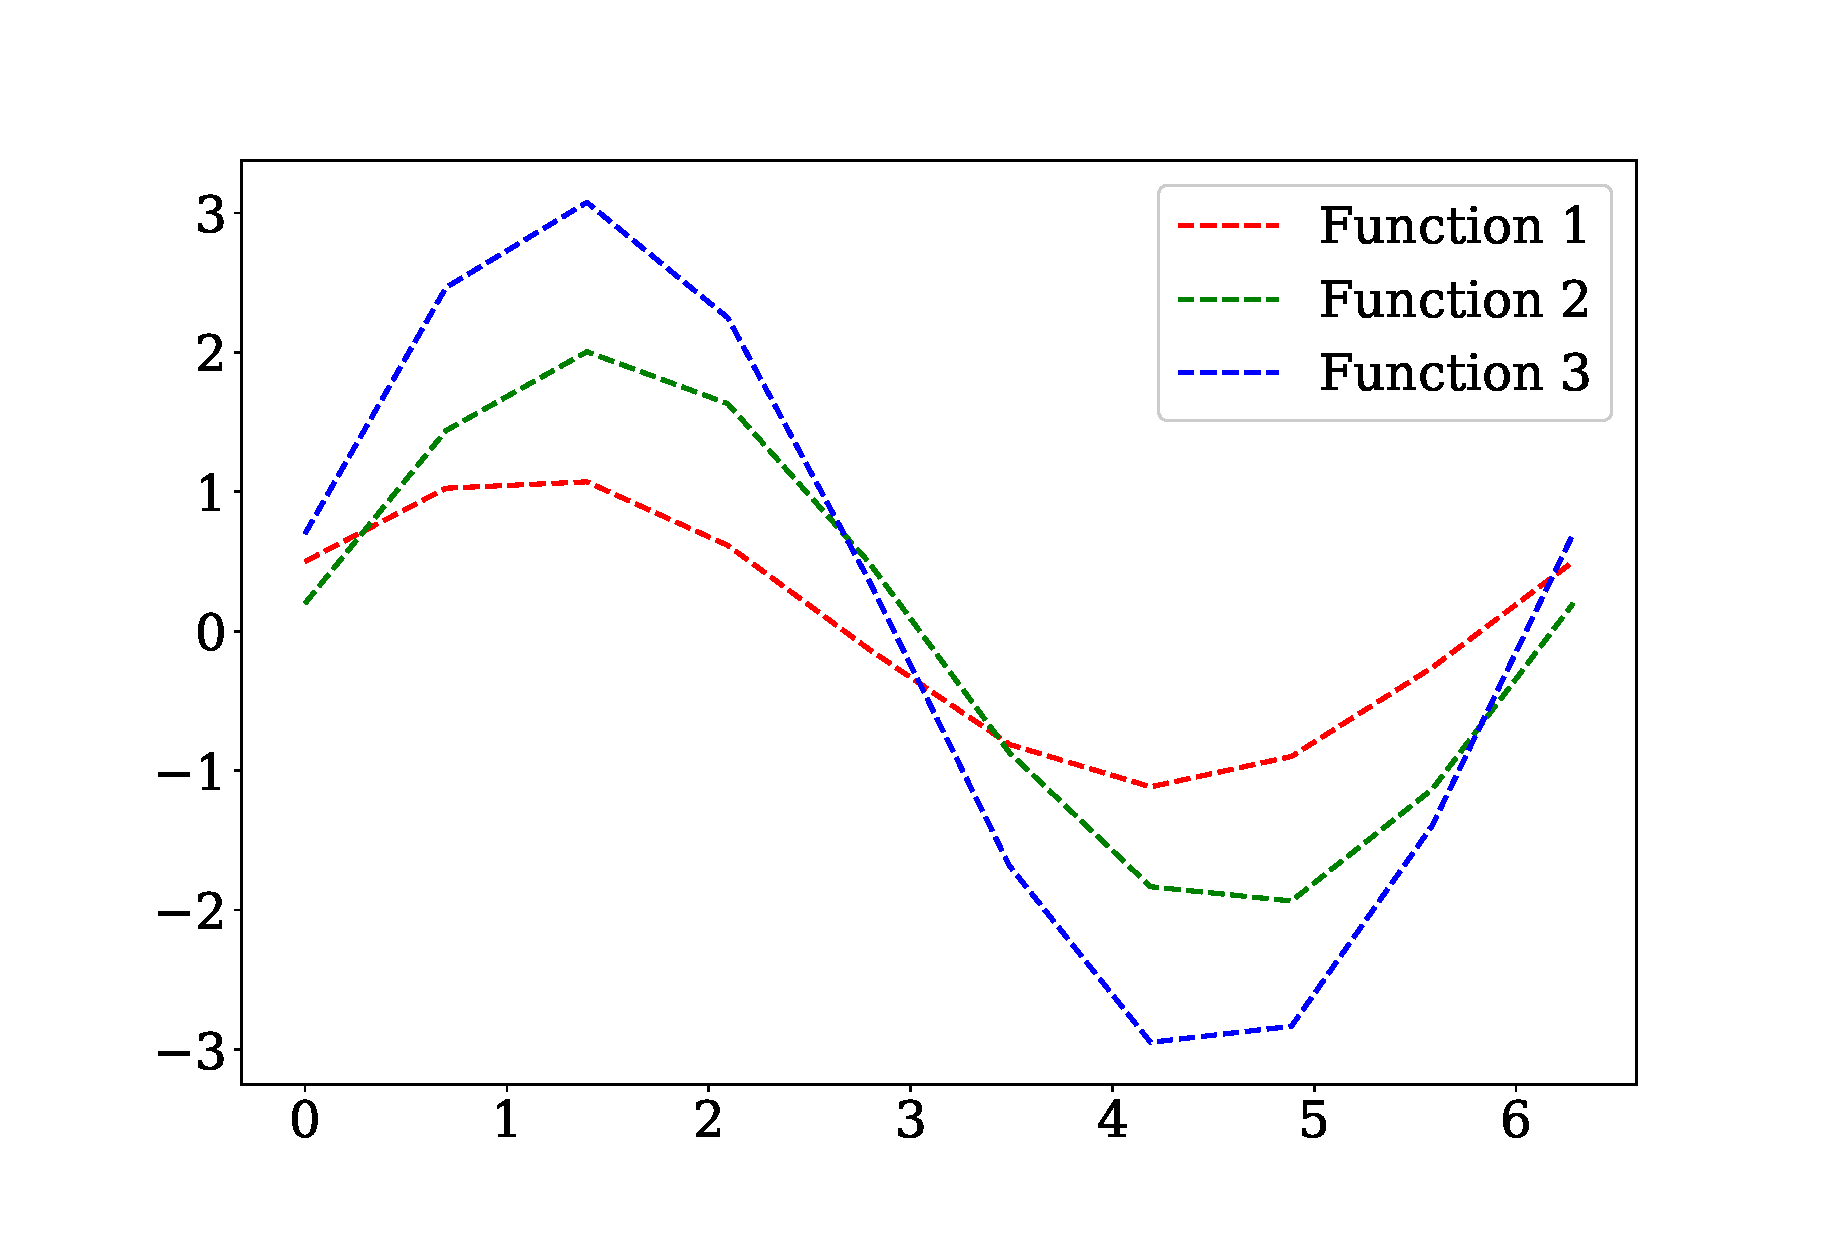
\includegraphics[width=0.5\textwidth]{Original_functions.eps}}
	\subfloat[Modified functions where 3 is subtracted from the last values]{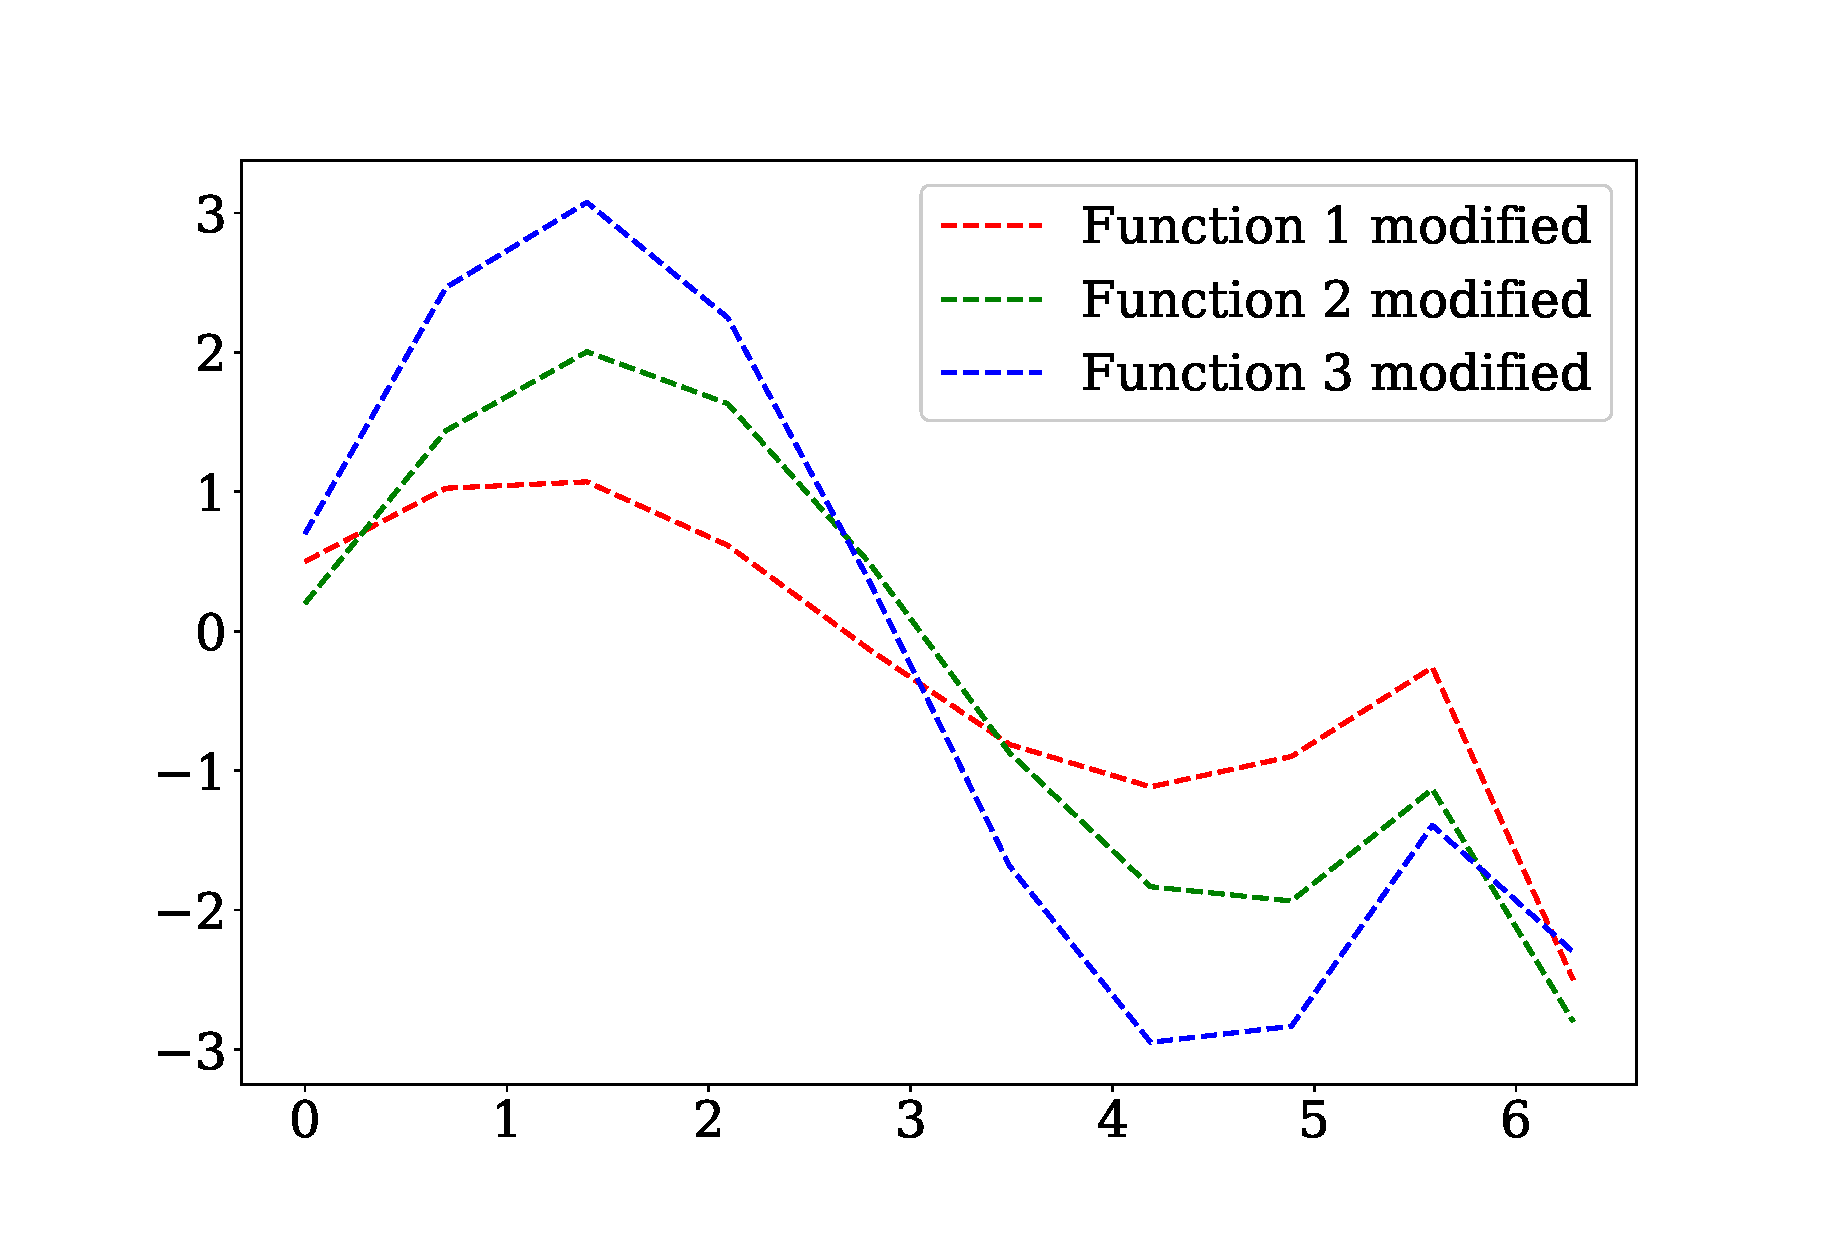
\includegraphics[width=0.5\textwidth]{Modified_functions.eps}}\\
	\caption{These sets of time series have the same distance matrix constructed on the Euclidean metric.}
	\label{fig:fig1}
\end{figure}

However, even using other metrics does not get rid of the problem. This results in the inability to use the classical Multidimentional Scaling \cite{MDS} algorithm to reconstruct the result to the source time series space. This algorithm is often used to reconstruct objects from their pairwise distances. Metric MDS Algorithm  \cite{inbook} may be used if distances are not euclidean.

In the theorem below we show that usage of only one matrix is insufficient for the problem of reconstructing values of time series.

\textbf{Theorem 1.} \emph{For any metric $\rho$ defined in the time series space $\mathbb{R}^t$ there is more than one way to reconstruct the original time series from the pairwise distance matrix constructed by the given metric.}	

\textbf{Note 1}. This statement does not use information about the first $t-1$ values of the series. In fact, the series in this case can be thought of as a point in $\mathbb{R}^t$ space. The usage of information about the previous moments of time is considered after this section.

\textbf{Proof}. We only have to show that the metric is not a bijection. This will mean that there are several different pairs of series whose distance between them is the same.

Let us show that the metric is a continuous function. Take the sequence \[\{(\mathbf{x}_n, \mathbf{y}_n)\} \subset \mathbb{R}^t \times \mathbb{R}^t, (\mathbf{x}_n, \mathbf{y}_n) \to (\mathbf{x}, \mathbf{y}).\] Then, \[\mathbf{x}_n\to \mathbf{x}, \mathbf{y}_n\to \mathbf{y} \Rightarrow \rho(\mathbf{x}_n,\mathbf{x})\to 0 ,\rho(\mathbf{y}_n,\mathbf{y})\to 0,\] $n \to \infty.$ Using the triangle inequality for the metric, we obtain \[\rho(\mathbf{x}_n,\mathbf{y}_n)\leqslant \rho(\mathbf{x}_n,\mathbf{x})+\rho(\mathbf{x},\mathbf{y})+\rho(\mathbf{y}_n,\mathbf{y})\to \rho(\mathbf{x},\mathbf{y}),\] therefore, $\rho(\mathbf{x}_n,\mathbf{y}_n)\to \rho(\mathbf{x},\mathbf{y})$.

Therefore the metric is a continuous mapping from $\mathbb{R}^t \times \mathbb{R}^t$ to $\mathbb{R}$. We will show that such a mapping cannot be a homeomorphism. Assume that $f: \mathbb{R} \to \mathbb{R}^t \times \mathbb{R}^t$ is the desired homeomorphism. Take arbitrary point $a \in \mathbb{R}$ and $f(a)$. Removing point $a$, $\mathbb{R}$ is no longer connected, but $\mathbb{R}^t \times \mathbb{R}^t$ is still connected. Therefore it is not a homeomorphism. We got a contradiction.
$\blacksquare$

\textbf{Note 2}. Essentially, the proof uses only the continuity of the function. This means that even non-metric continuous functions will give the multiplicity of the answer. For example, pairwise correlation of series is also a continuous function.

Thus, knowing only the distance matrix it is impossible to unambiguously reconstruct the original series.

Now consider the same problem, in addition to the matrix $\mathbf{\Sigma}_{t+1}$ using the value of the time series before the time moment $t$: $\mathbf{X}=[\mathbf{x_1}, \ldots, \mathbf{x_{t}}]$. The problem is reformulated as follows:

There are $n$ objects in $\mathbb{R}^{t+1}$, their first $t$ coordinates are known. We also know the distance matrix $\mathbf{\Sigma}_{t+1} \in \mathbb{R}^{(t+1) \times (t+1)}$. It is required to calculate the ($t+1$)'th coordinate of each of the objects. In time series terms, the ($t+1$)'th coordinate is the value of each of the series at that moment in time.

\section{Pairwise correlation between time series}

In this section we investigates the time series values reconstruction using the pairwise correlation matrix. This distance function is used because it is shown in the article \cite{puchkin2023sharper} that the pairwise correlation estimate of a sample approximates its mathematical expectation.

The pairwise distance matrix is constructed as follows:
\begin{gather*}
	{\mathbf{\Sigma}}_T = \frac{1}{T} \sum_{t=1}^{T} (\mathbf{x}_t - \boldsymbol{\mu}_T)(\mathbf{x}_t - \boldsymbol{\mu}_T)^\mathsf{T},\\
	\boldsymbol{\mu}_T = \frac{1}{T} \sum_{t=1}^{T} \mathbf{x}_t.
\end{gather*}

\textbf{Theorem 2.} \emph{In the case of accurately predicted distance matrix, the function} $||\hat{\mathbf{\Sigma}}_{t+1} - \bar{\mathbf{\Sigma}}_{t+1}||_2^2$ \emph{will have two minimums, defined explicitly as follows:}

\begin{align*}
	\hat{\mathbf{y}}_i &= \mathbf{y}_i,\\
	\hat{\mathbf{y}}_i &= \frac{2}{T-1} \sum_{k=1}^{T-1} \mathbf{a}_{ik} - \mathbf{y}_i,
\end{align*}
\emph{where} $\hat{\mathbf{y}}_i$ $i$\emph{-th coordinate of the predicted value of the series at the moment $T+1$, $\mathbf{A}=(\mathbf{a}_{ik})$ is given multivariate time series,} $y_i$ \emph{are true values of the series at the moment} $T+1$.

\textbf{Proof.} Let us denote by $\mathbf{\Sigma}$ the true matrix at the moment of time $T$, and $\hat{\mathbf{\Sigma}}$ the predicted one. By construction, ${\mathbf{\Sigma}} = \frac{1}{T} \sum_{k=1}^{T} (\mathbf{a}^T_k - \boldsymbol{\mu}_T)(\mathbf{a}^T_k - \boldsymbol{\mu}_T)^\intercal\texttt{}$. The matrix $\mathbf{A}$ is a transposed matrix $\mathbf{X}$ of time series, where the first dimension is the number of the series, not the moment of time as in the case of $\mathbf{X}$. Then, consider what the elements of the matrices $\mathbf{\Sigma}$ and $\hat{\mathbf{\Sigma}}$ are equal to.
\begin{align*}
	&\mathbf{\Sigma}_{ij} = \frac{1}{T}\sum_{k=1}^{T}(\mathbf{a}_{ik} - \boldsymbol{\mu}_i)(\mathbf{a}_{jk}-\boldsymbol{\mu}_j),\\
    &\text{separating last term,}\\
	&\hat{\mathbf{\Sigma}}_{ij} = \frac{1}{T}\sum_{k=1}^{T-1}(\mathbf{a}_{ik} - \hat{\boldsymbol{\mu}}_i)(\mathbf{a}_{jk}-\hat{\boldsymbol{\mu}}_j) + (\mathbf{y}_i - \hat{\boldsymbol{\mu}}_i)(\mathbf{y}_j - \hat{\boldsymbol{\mu}}_j).
\end{align*}

Since we minimise the norm of the difference, both matrices are equal to each other. Consider the equality of diagonal elements.
\begin{gather*}
	\text{For any } i, j \text{ such that } i = j \text{ the following is true: } \mathbf{\Sigma}_{ii} = \hat{\mathbf{\Sigma}}_{ii},\\
	\sum_{k=1}^{T}(\mathbf{a}_{ik} - \boldsymbol{\mu}_i)(\mathbf{a}_{ik}-\boldsymbol{\mu}_i) = \sum_{k=1}^{T-1}(\mathbf{a}_{ik} - \hat{\boldsymbol{\mu}}_i)(\mathbf{a}_{ik}-\hat{\boldsymbol{\mu}}_i) + (\mathbf{y}_i - \hat{\boldsymbol{\mu}}_i)(\mathbf{y}_i - \hat{\boldsymbol{\mu}}_i),\\
	\text{since } \boldsymbol{\mu}_i \text{ and } \hat{\boldsymbol{\mu}}_i \text{ are equal up to } (T-1) \text{-th coordinate,}\\
	(\mathbf{a}_{iT}-\boldsymbol{\mu}_i)^2 = (\mathbf{y}_i-\hat{\boldsymbol{\mu}}_i)^2.\\
	\text{Consider } \hat{\boldsymbol{\mu}}_i \text{ and } \hat{\boldsymbol{\mu}}:\\
	\hat{\boldsymbol{\mu}}_i = \frac{1}{T}\sum_{k=1}^{T-1}\mathbf{a}_{ik} + \frac{1}{T}\mathbf{y}_i,\\
	\boldsymbol{\mu}_i = \frac{1}{T}\sum_{k=1}^{T}\mathbf{a}_{ik}.\\
	\text{Substitute the expressions for } \hat{\boldsymbol{\mu}} \text{ into } (\mathbf{a}_{iT}-\boldsymbol{\mu}_i)^2 = (\mathbf{y}_i-\hat{\boldsymbol{\mu}}_i)^2:\\
	\left[
	\begin{array}{ll}
		\frac{T-1}{T}\mathbf{y}_i-\frac{1}{T}\sum_{k=1}^{T-1}\mathbf{a}_{ik}=\mathbf{a}_{iT}-\boldsymbol{\mu}_i
		\\[1ex]
		\frac{T-1}{T}\mathbf{y}_i-\frac{1}{T}\sum_{k=1}^{T-1}\mathbf{a}_{ik}=\boldsymbol{\mu}_i-\mathbf{a}_{iT}
	\end{array},
	\right .\\[1ex]
	\text{Rewriting } \boldsymbol{\mu} \text{,}\\
	\left[
	\begin{array}{ll}
		\frac{T-1}{T}\mathbf{y}_i = \frac{T-1}{T}\mathbf{a}_{iT}
		\\[1ex]
		\frac{T_1}{T}\mathbf{y}_i = \frac{2}{T} \sum_{k=1}^{T-1} \mathbf{a}_{ik} - \frac{T-1}{T}\mathbf{a}_{iT}
	\end{array},
	\right .\\[1ex]
	\left[
	\begin{array}{ll}
		\mathbf{y}_i = \mathbf{a}_{iT}
		\\[1ex]
		\mathbf{y}_i = \frac{2}{T-1} \sum_{k=1}^{T-1} \mathbf{a}_{ik} - \mathbf{a}_{iT}
	\end{array}.
	\right .
\end{gather*}

Redefining, we obtain
\begin{align*}
	\hat{\mathbf{y}_i} &= \mathbf{y}_i,\\
	\hat{\mathbf{y}_i} &= \frac{2}{T-1} \sum_{k=1}^{T-1} \mathbf{a}_{ik} - \mathbf{y}_i.
\end{align*}
$$ \blacksquare $$

Figure \ref{fig:fig2} shows an example of a function $||\hat{\mathbf{\Sigma}}_{t+1} - \bar{\mathbf{\Sigma}}_{t+1}||_2^2$ with two minimum for certain time series.

\textbf{Corollary. (A trivial method for obtaining a pair of possible answers.)} This theorem shows that using pairwise correlation as a distance function gives at most \emph{two} different answers when reconstructing. Moreover, having obtained one, we can explicitly find the second one. Then, to find both possible answers, it is proposed to apply any non-convex optimisation method to find at least one of the minimum of the function. Therefore with the formula above we are able to find another minimum.

\begin{figure}[!htbp]
	\centering
	\begin{center}
		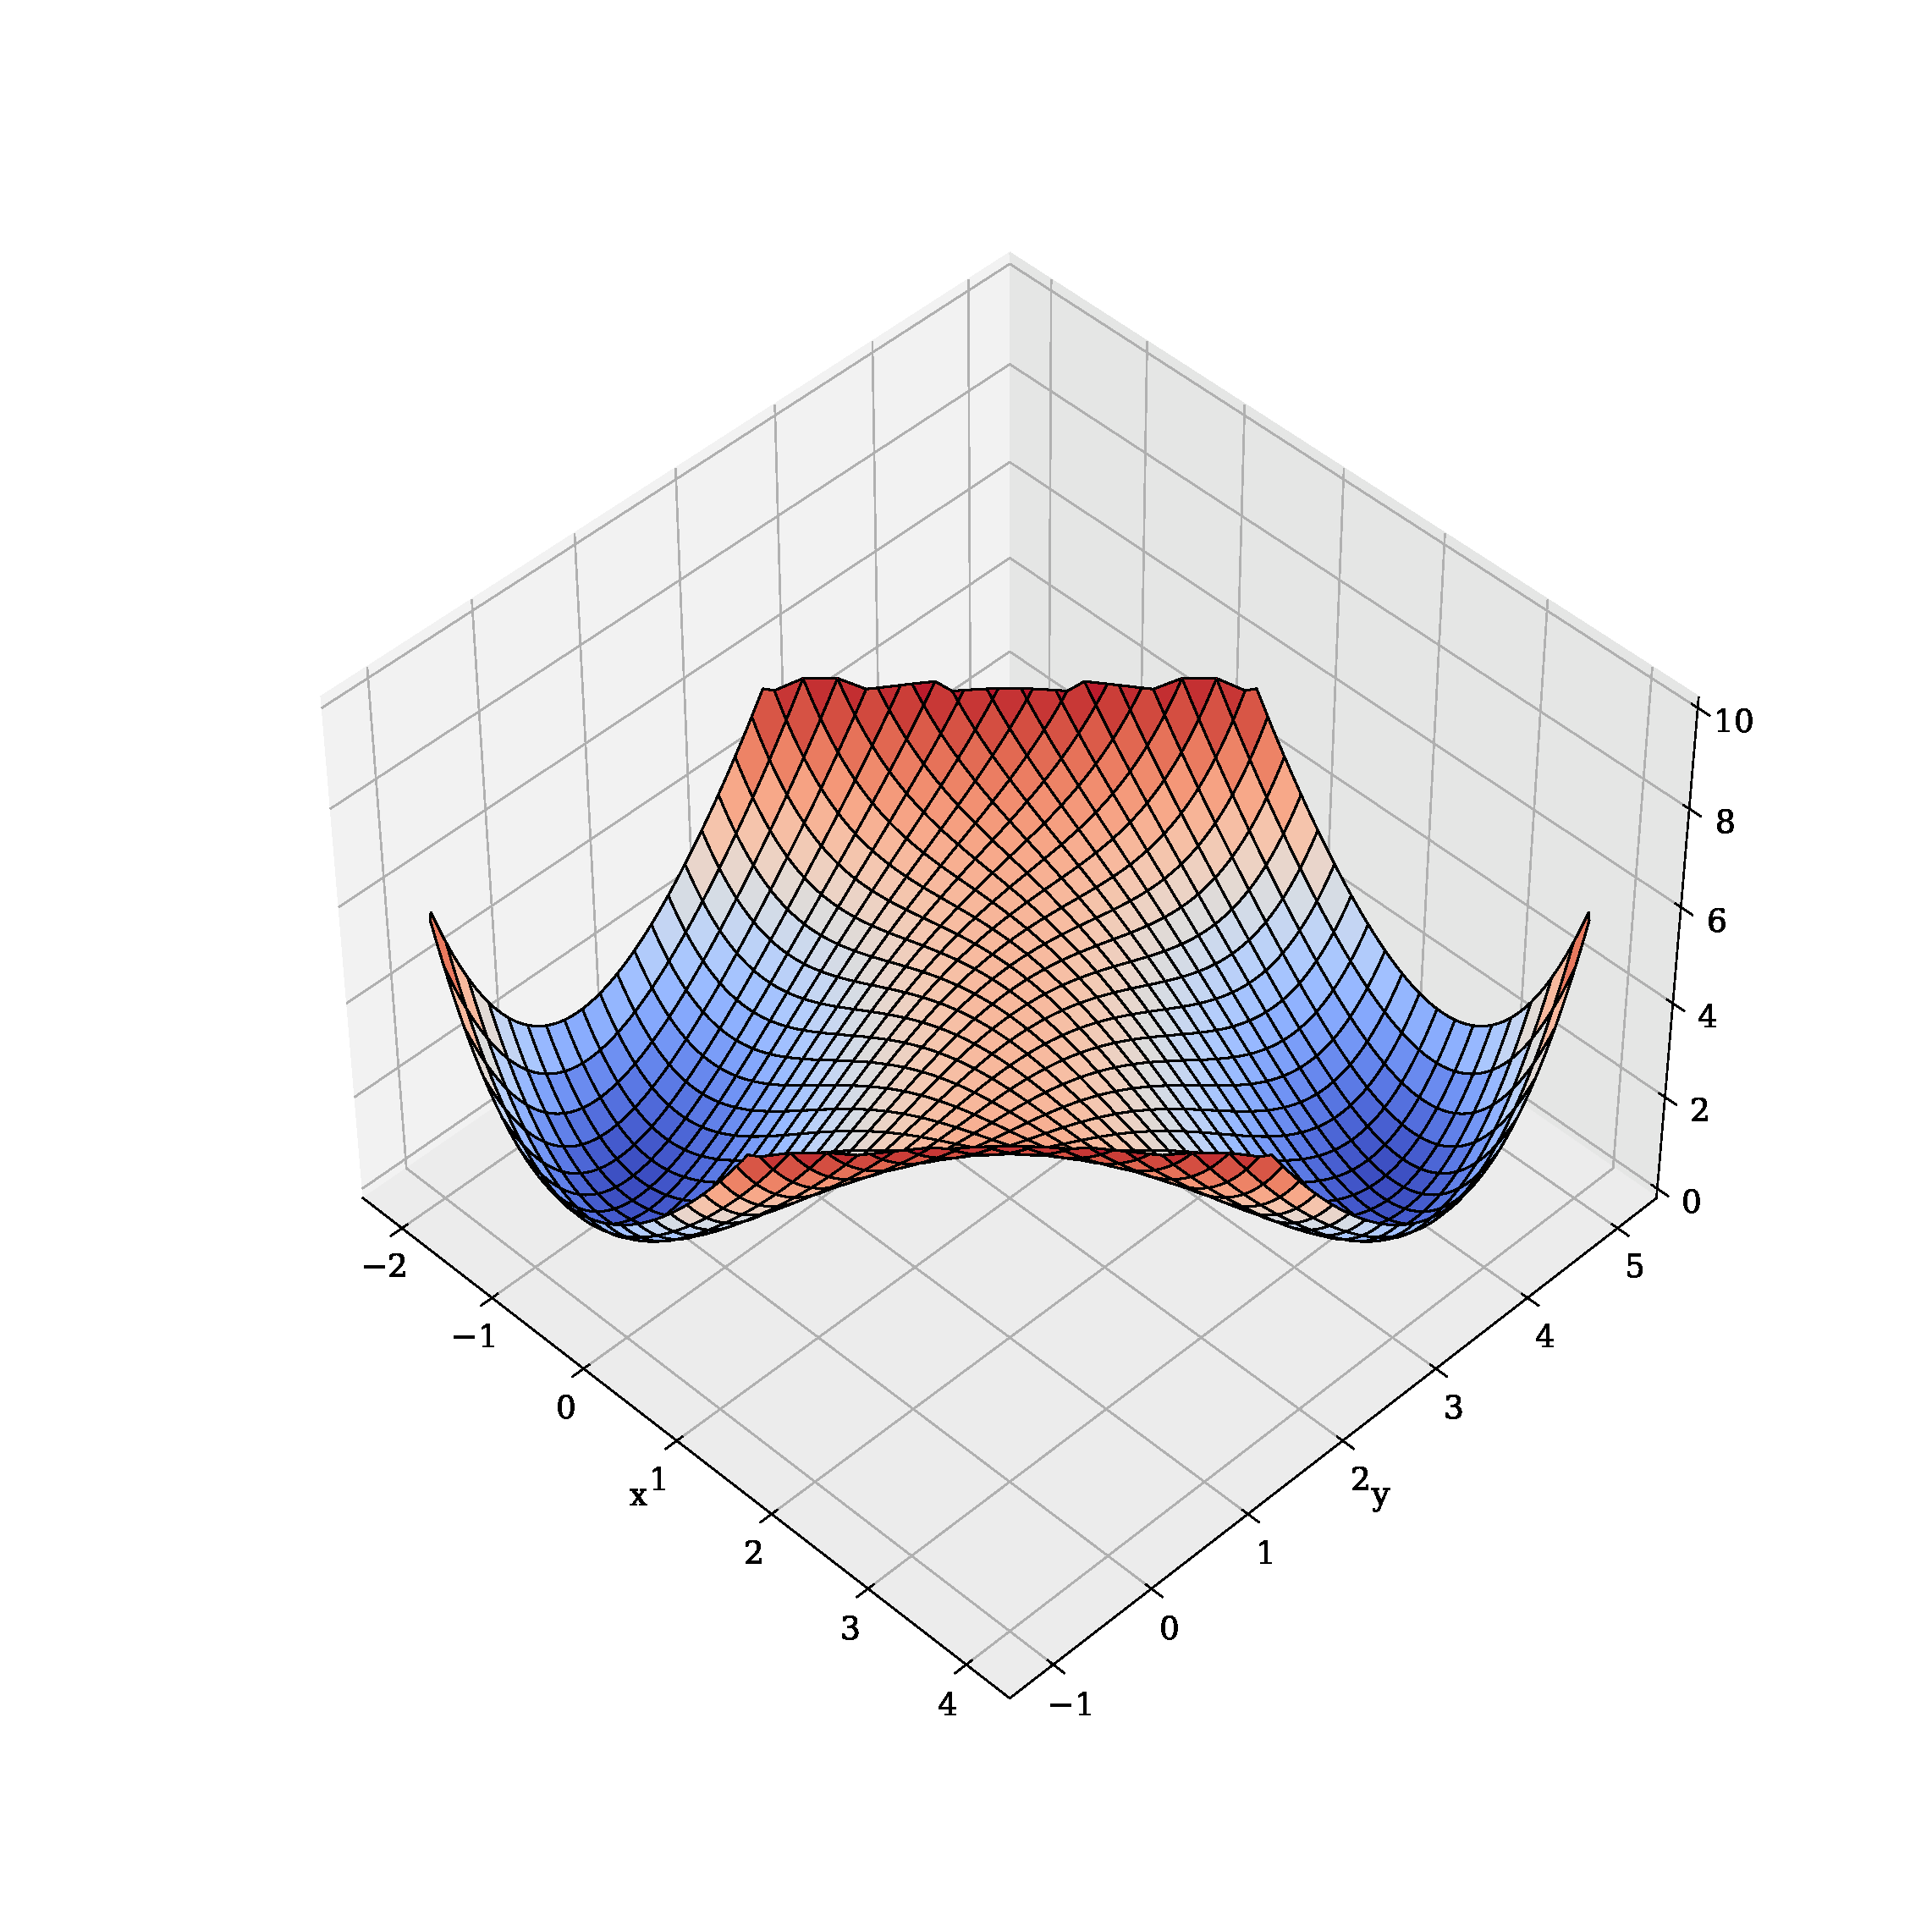
\includegraphics[width=0.8\textwidth]{NonConvex.eps}
	\end{center}
	\caption{Function $||\hat{\mathbf{\Sigma}}_{t+1} - \bar{\mathbf{\Sigma}}_{t+1}||_2^2$ for following series: $(1, 3)$ and $(2, 4)$. Minumums: (3; 4) is desired and (-1; 0) is alternative.}
	\label{fig:fig2}
\end{figure}


The problem with this method is the computational cost of non-convex optimisation methods. As an alternative, we propose the following method using only singular matrix decomposition.

{\textbf{Theorem 3. (Efficient method for obtaining a pair of possible answers.)} \emph{ The minimum of the function $||\hat{\mathbf{\Sigma}}_{t+1} - \bar{\mathbf{\Sigma}}_{t+1}||_2^2$ is reached on \[\pm\sqrt{\lambda_1} \mathbf{u}_1 + \boldsymbol{\mu}_t,\] where $\lambda_1$ is the first singular value, $\mathbf{u}_1$ is the first left singular vector of matrix $\mathbf{A}=\left(\hat{\mathbf{\Sigma}}_{t+1} - \frac{t}{t+1} \cdot \mathbf{\Sigma}_t \right) \cdot \frac{(t+1)^2}{t}$}

\textbf{Proof.} The notation $\mathbf{x}_i$ is used below to denote the \emph{multidimensional} value of the time series at time $i$. The proof expresses $\mathbf{\Sigma}_{t+1}$ through $\mathbf{\Sigma}_t$. After that, the operator norm and rank property of the matrix is used. All expressions below are true for arbitrary $\boldsymbol{\mu}_T$ and $\mathbf{\Sigma}_T$ constructed by the definition above.
\begin{enumerate}
	\item Express $\boldsymbol{\mu}$ through the values of the time series: \[\boldsymbol{\mu}_t = \frac{1}{t} \sum_{i=1}^{t} \mathbf{x}_i \Rightarrow \sum_{i=1}^{t} \mathbf{x}_i = t \boldsymbol{\mu}_t.\]
	\item Similarly, express $\mathbf{\Sigma_t}$ through the values of the series:
		\begin{gather*}
		\mathbf{\Sigma}_t = \frac{1}{t} \sum_{i=1}^{t} (\mathbf{x}_i-\boldsymbol{\mu}_t)(\mathbf{x}_i-\boldsymbol{\mu}_t)^\intercal;\\
		\mathbf{\Sigma}_t = \frac{1}{t} \sum_{i=1}^{t} \mathbf{x}_i \mathbf{x}_i^\intercal - \frac{1}{t} \left( \sum_{i=1}^{t} \mathbf{x}_i\right) \boldsymbol{\mu}_t^\intercal - \boldsymbol{\mu}_t \frac{1}{t} \left( \sum_{i=1}^{t} \mathbf{x}_i^\intercal\right) + \boldsymbol{\mu}_t \boldsymbol{\mu}_t^\intercal =\\= \frac{1}{t} \sum_{i=1}^{t} \mathbf{x}_i \mathbf{x}_i^\intercal - \boldsymbol{\mu}_t \boldsymbol{\mu}_t^\intercal \Rightarrow\\
		\sum_{i=1}^{t} \mathbf{x}_i \mathbf{x}_i^\intercal = t \mathbf{\Sigma}_t + t \boldsymbol{\mu}_t \boldsymbol{\mu}_t^\intercal.
		\end{gather*}
	\item Express $\mathbf{\Sigma_{t+1}}$ with $\mathbf{\Sigma_t}$ using the previous expressions:
	\begin{gather*}
		\mathbf{\Sigma}_{t+1} = \frac{1}{t+1} \left(\sum_{i=1}^{t} \mathbf{x}_i \mathbf{x}_i^\intercal + \mathbf{x}_{t+1} \mathbf{x}_{t+1}^\intercal \right) - \boldsymbol{\mu}_{t+1} \boldsymbol{\mu}_{t+1}^\intercal = \\
		= \frac{t}{t+1}\mathbf{\Sigma}_t + \frac{t}{t+1}\boldsymbol{\mu}_{t} \boldsymbol{\mu}_{t}^\intercal + \frac{1}{t+1} \mathbf{x}_{t+1} \mathbf{x}_{t+1}^\intercal - \frac{1}{(t+1)^2} (t \boldsymbol{\mu}_t + \mathbf{x}_{t+1})(t \boldsymbol{\mu}_t + \mathbf{x}_{t+1})^\intercal =\\
		= \frac{t}{t+1}\mathbf{\Sigma}_t + \frac{t}{t+1}\boldsymbol{\mu}_{t} \boldsymbol{\mu}_{t}^\intercal + \frac{t}{(t+1)^2} \mathbf{x}_{t+1} \mathbf{x}_{t+1}^\intercal -\\- \frac{t^2}{(t+1)^2}\boldsymbol{\mu}_{t} \boldsymbol{\mu}_{t}^\intercal - \frac{t}{(t+1)^2}\boldsymbol{\mu}_{t} \mathbf{x}_{t+1}^\intercal - \frac{t}{(t+1)^2}\mathbf{x}_{t+1} \boldsymbol{\mu}_{t}^\intercal =\\
		= \frac{t}{t+1}\mathbf{\Sigma}_t + \frac{t}{t+1}\boldsymbol{\mu}_{t} \boldsymbol{\mu}_{t}^\intercal - \frac{t}{(t+1)^2} \left( -\mathbf{x}_{t+1} \mathbf{x}_{t+1}^\intercal + t\boldsymbol{\mu}_{t} \boldsymbol{\mu}_{t}^\intercal + \boldsymbol{\mu}_{t} \mathbf{x}_{t+1}^\intercal + \mathbf{x}_{t+1} \boldsymbol{\mu}_{t}^\intercal \right) =\\
		= \frac{t}{t+1}\mathbf{\Sigma}_t + \frac{t}{t+1}\boldsymbol{\mu}_{t} \boldsymbol{\mu}_{t}^\intercal - \frac{t}{(t+1)^2} \left( -(\mathbf{x}_{t+1}-\boldsymbol{\mu}_t)(\mathbf{x}_{t+1}-\boldsymbol{\mu}_t)^\intercal + (t+1)\boldsymbol{\mu}_{t} \boldsymbol{\mu}_{t}^\intercal \right) =\\
		= \frac{t}{t+1}\mathbf{\Sigma}_t + \frac{t}{t+1}\boldsymbol{\mu}_{t} \boldsymbol{\mu}_{t}^\intercal - \frac{t(t+1)}{(t+1)^2}\boldsymbol{\mu}_{t} \boldsymbol{\mu}_{t}^\intercal + \frac{t}{(t+1)^2}(\mathbf{x}_{t+1}-\boldsymbol{\mu}_t)(\mathbf{x}_{t+1}-\boldsymbol{\mu}_t)^\intercal =\\
		= \frac{t}{t+1}\mathbf{\Sigma}_t + \frac{t}{(t+1)^2}(\mathbf{x}_{t+1}-\boldsymbol{\mu}_t)(\mathbf{x}_{t+1}-\boldsymbol{\mu}_t)^\intercal.
	\end{gather*}
	This equality expresses $\mathbf{\Sigma}_{t+1}$ through $\mathbf{\Sigma}_t$. For further proof it is useful to derive the following equality for our problem: \[(\bar{\mathbf{x}}_{t+1}-\boldsymbol{\mu}_t)(\bar{\mathbf{x}}_{t+1}-\boldsymbol{\mu}_t)^\intercal = \left(\bar{\mathbf{\Sigma}}_{t+1} - \frac{t}{t+1} \cdot \mathbf{\Sigma}_t \right) \cdot \frac{(t+1)^2}{t}.\]
	
	\item We solve the problem of finding the minimum of the function $||\hat{\mathbf{\Sigma}}_{t+1} - \bar{\mathbf{\Sigma}}_{t+1}||_2^2$. In our case, this is analogous to the equality of this function to zero. Let us write the expression under the norm:
	\begin{gather*}
		\hat{\mathbf{\Sigma}}_{t+1} - \bar{\mathbf{\Sigma}}_{t+1} = \frac{t}{t+1}\mathbf{\Sigma}_t + \frac{t}{(t+1)^2}(\hat{\mathbf{x}}_{t+1}-\boldsymbol{\mu}_t)(\hat{\mathbf{x}}_{t+1}-\boldsymbol{\mu}_t)^\intercal -\\- \frac{t}{t+1}\mathbf{\Sigma}_t + \frac{t}{(t+1)^2}(\bar{\mathbf{x}}_{t+1}-\boldsymbol{\mu}_t)(\bar{\mathbf{x}}_{t+1}-\boldsymbol{\mu}_t)^\intercal =\\
		=\frac{t}{(t+1)^2}(\hat{\mathbf{x}}_{t+1}-\boldsymbol{\mu}_t)(\hat{\mathbf{x}}_{t+1}-\boldsymbol{\mu}_t)^\intercal -\frac{t}{(t+1)^2}(\bar{\mathbf{x}}_{t+1}-\boldsymbol{\mu}_t)(\bar{\mathbf{x}}_{t+1}-\boldsymbol{\mu}_t)^\intercal.
 	\end{gather*}
 	Then, the problem above is equivalent to finding the minimum of the function \[||(\hat{\mathbf{x}}_{t+1}-\boldsymbol{\mu}_t)(\hat{\mathbf{x}}_{t+1}-\boldsymbol{\mu}_t)^\intercal-(\bar{\mathbf{x}}_{t+1}-\boldsymbol{\mu}_t)(\bar{\mathbf{x}}_{t+1}-\boldsymbol{\mu}_t)^\intercal||_2^2.\]
 	Denote \[\mathbf{A} = (\bar{\mathbf{x}}_{t+1}-\boldsymbol{\mu}_t)(\bar{\mathbf{x}}_{t+1}-\boldsymbol{\mu}_t)^\intercal = \left(\bar{\mathbf{\Sigma}}_{t+1} - \frac{t}{t+1} \cdot \mathbf{\Sigma}_t \right) \cdot \frac{(t+1)^2}{t}.\]
 	The rank of the matrix ($\hat{\mathbf{x}}_{t+1}-\boldsymbol{\mu}_t)(\hat{\mathbf{x}}_{t+1}-\boldsymbol{\mu}_t)^\intercal$ is 1, and since the desired minimum is 0, it turns out that the rank of the matrix $\mathbf{A}$ is also 1.
 	
 	\item From the previous paragraph, the matrix $\mathbf{A}$ has rank 1. Consider the singular value decomposition. \[
 		\mathbf{A} = \sum_{i=1}^{1} \lambda_i \mathbf{u}_i \mathbf{v}_i^\intercal = \lambda_1 \mathbf{u}_1 \mathbf{v}_1^\intercal.
 	\]
 	On the other hand, $\mathbf{A} = (\bar{\mathbf{x}}_{t+1}-\boldsymbol{\mu}_t)(\bar{\mathbf{x}}_{t+1}-\boldsymbol{\mu}_t)^\intercal$. Then, \[
 	\bar{\mathbf{x}}_{t+1}-\boldsymbol{\mu}_t = \pm\sqrt{\lambda_1} \mathbf{u}_1 \Leftrightarrow\\
 	\bar{\mathbf{x}}_{t+1} = \pm\sqrt{\lambda_1} \mathbf{u}_1 + \boldsymbol{\mu}_t.
 	\]
 	The sign $\pm$ comes from the fact that in the case of a symmetric matrix, there are two singular value decompositions: $\mathbf{A}=\mathbf{U}\mathbf{\Sigma} \mathbf{V}^\intercal=(-\mathbf{U})\mathbf{\Sigma} (-\mathbf{V})^\intercal$.
 	$$ \blacksquare $$
\end{enumerate}

This theorem allows us to find both minimums of a function much faster than with standard non-convex optimisation methods \cite{mikhalevich2024methodsnonconvexoptimization}.

\section{Algorithm for reconstructing time series values in case of accurate prediction of the matrix}

Theorems 2 and 3 show that using a \emph{single} pairwise correlation matrix and information about the first $t$ moments of time allows us to obtain a \emph{pair} of possible values after recovery. In this section, we propose a method to select the true value from the obtained \emph{pair} $\mathbf{\Sigma}_{t+1}$ \emph{predicted accurately}.

The algorithm described below is based on the use of \emph{two} predicted matrices corresponding to different subsegments of time. Two different values $T, T^\prime$ are chosen. Two matrices are predicted:

First matrix $\mathbf{\Sigma}_{t+1}^1$ pairwise correlation matrix for the multivariate time series $\mathbf{x}$ at time moments from $t-T+2$ to $t+1$ (in total $T$ values).

Second matrix $\mathbf{\Sigma}_{t+1}^2$ pairwise correlation matrix for the multivariate time series $\mathbf{x}$ at time moments from $t-T‘+2$ to $t+1$ (in total $T^\prime$ values).

Hence, when we reconstruct answers from these matrices, we obtain two pairs of answers, each of which is a candidate for the true answer. At the same time, a true answer exists in each of the pairs. We suggest to take the answer from the intersection. We does not consider the case when the intersection size is 2, since the probability of this situation is 0 when using continuous values.

Algorithm scheme:

\begin{enumerate}
	\item Take $T$ and $T^\prime: T \neq T'$.
	\item For $T$ and $T^\prime$ perform the above algorithm and obtain the answer sets: 
	\begin{gather*}
	 [\hat{\mathbf{x}}_{t+1}^1, \hat{\mathbf{x}}^{\prime 1}_{t+1}],\\ [\hat{\mathbf{x}}_{t+1}^2, \hat{\mathbf{x}}^{\prime 2}_{t+1}].
	 \end{gather*}
	\item Find the answer that lies in the intersection.
	In real data, the probability of matching sets of answers is 0, just as it is in synthetic data with random noise added.
\end{enumerate}

\ref{fig:fig3} shows the example of reconstructed time series with accurate predicted matrix. As you can see in the graph, the reconstruction is lossless.

\begin{figure}[!htbp]
	\centering
	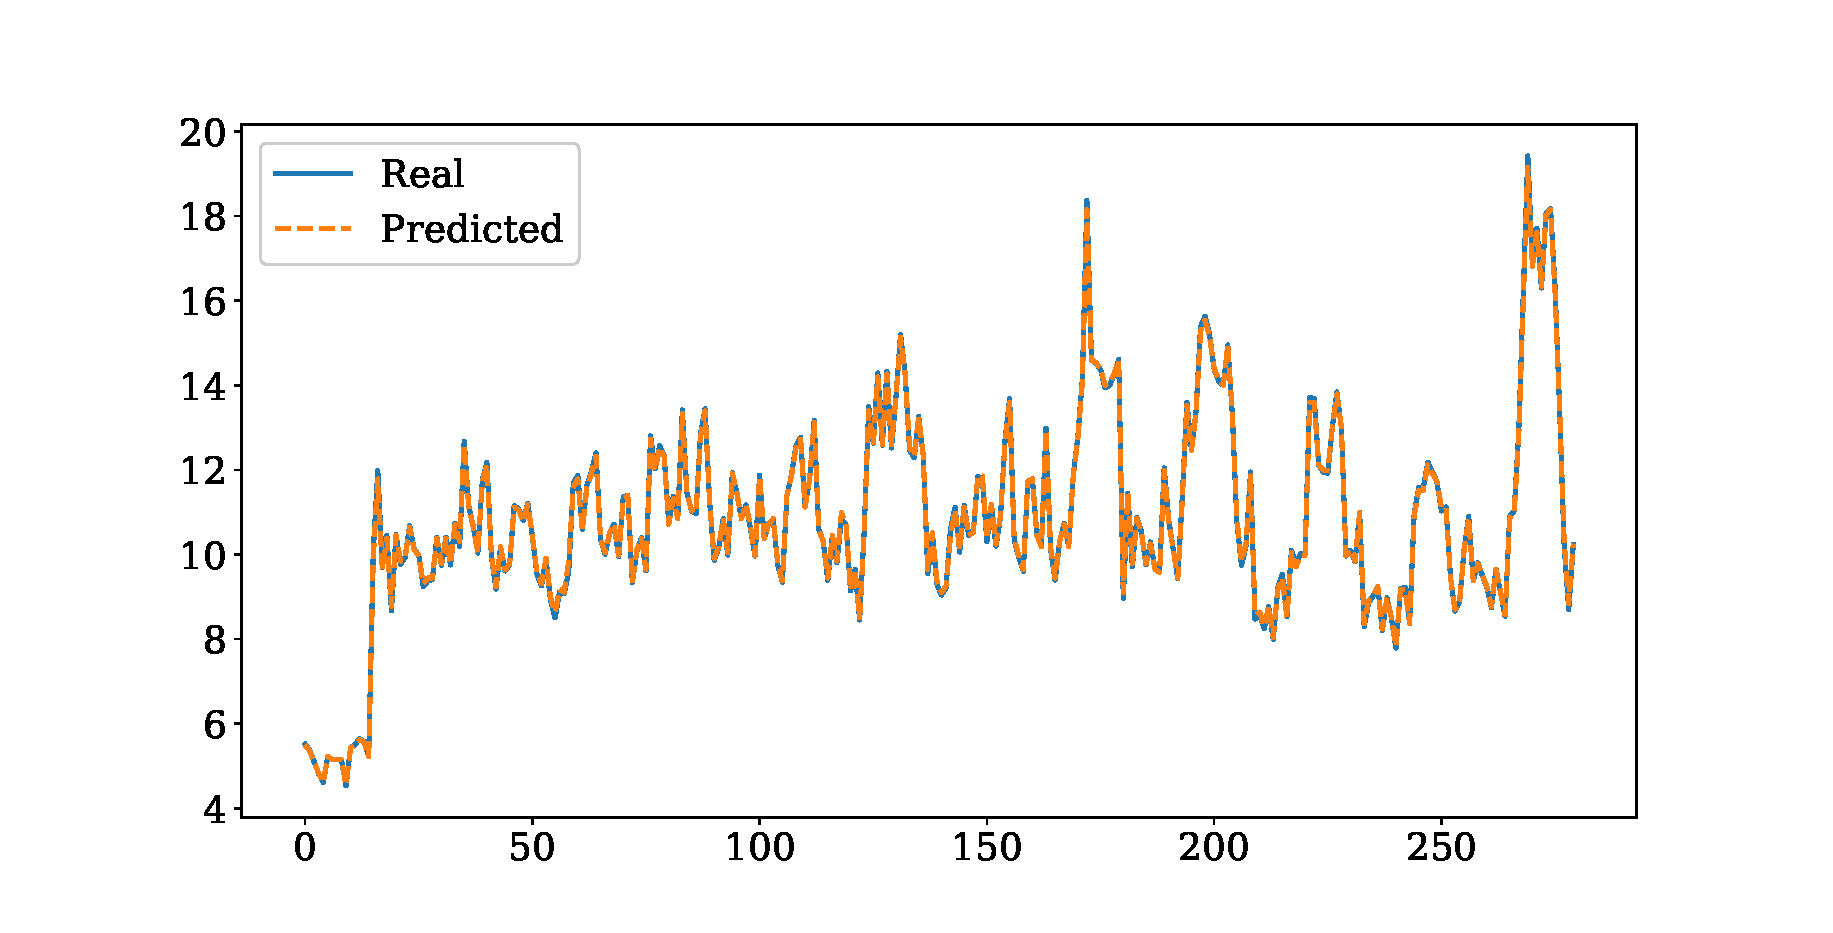
\includegraphics[width=\textwidth]{IdealRecovery.eps}
	\caption{Prediction recovery in case of accurate prediction of correlation matrix $\mathbf{\Sigma}$. $T=20$, $T^\prime=10$}
	\label{fig:fig3}
\end{figure}

\section{Algorithm for reconstructing time series values in case of inaccurate matrix prediction}

The problem with the above algorithm is that if the prediction is inaccurate, there may be no intersection. This happens because the error in each of the predicted matrices is different. For this, the following algorithm is proposed to amortise the error:

Instead of two values of $T$ and $T^\prime$, we propose take $K$ values. We get $K$ matrices with some noise that came from inaccuracy in prediction. Thus, each matrix is reduced to the nearest positive semi-definite matrix. Algorithm is explained in \cite{HIGHAM1988103}.
Then, for each value algorithm for obtaining the pair of possible answers is applied.

We get $K$ sets of answers:
\begin{gather*}
	[\hat{\mathbf{x}}_{t+1}^1, \hat{\mathbf{x}}^{\prime 1}_{t+1}],\\
	[\hat{\mathbf{x}}_{t+1}^2, \hat{\mathbf{x}}^{\prime 2}_{t+1}],\\
	\vdots \\
	[\hat{\mathbf{x}}_{t+1}^K, \hat{\mathbf{x}}^{\prime K}_{t+1}].
\end{gather*}
Then we propose to search through $2^K$ sets of answers and choose the set in which the diameter is minimal. The diameter of set is calculated as maximum Euclidean distance between two different points in set. It is a \emph{necessary} condition for the actual answer. In the case of an accurate prediction, the diameter of such a set will always be zero.

The asymptotic complexity of this reconstruction will be $O(2^K \times K \times N)$ $+$ the complexity of the minimum search algorithm used.

On \ref{fig:fig4} you can see an example of reconstructing time series values when the predicted matrix contains some random noise. The reconstruction is no more lossless.

\begin{figure}[!htbp]
	\centering
	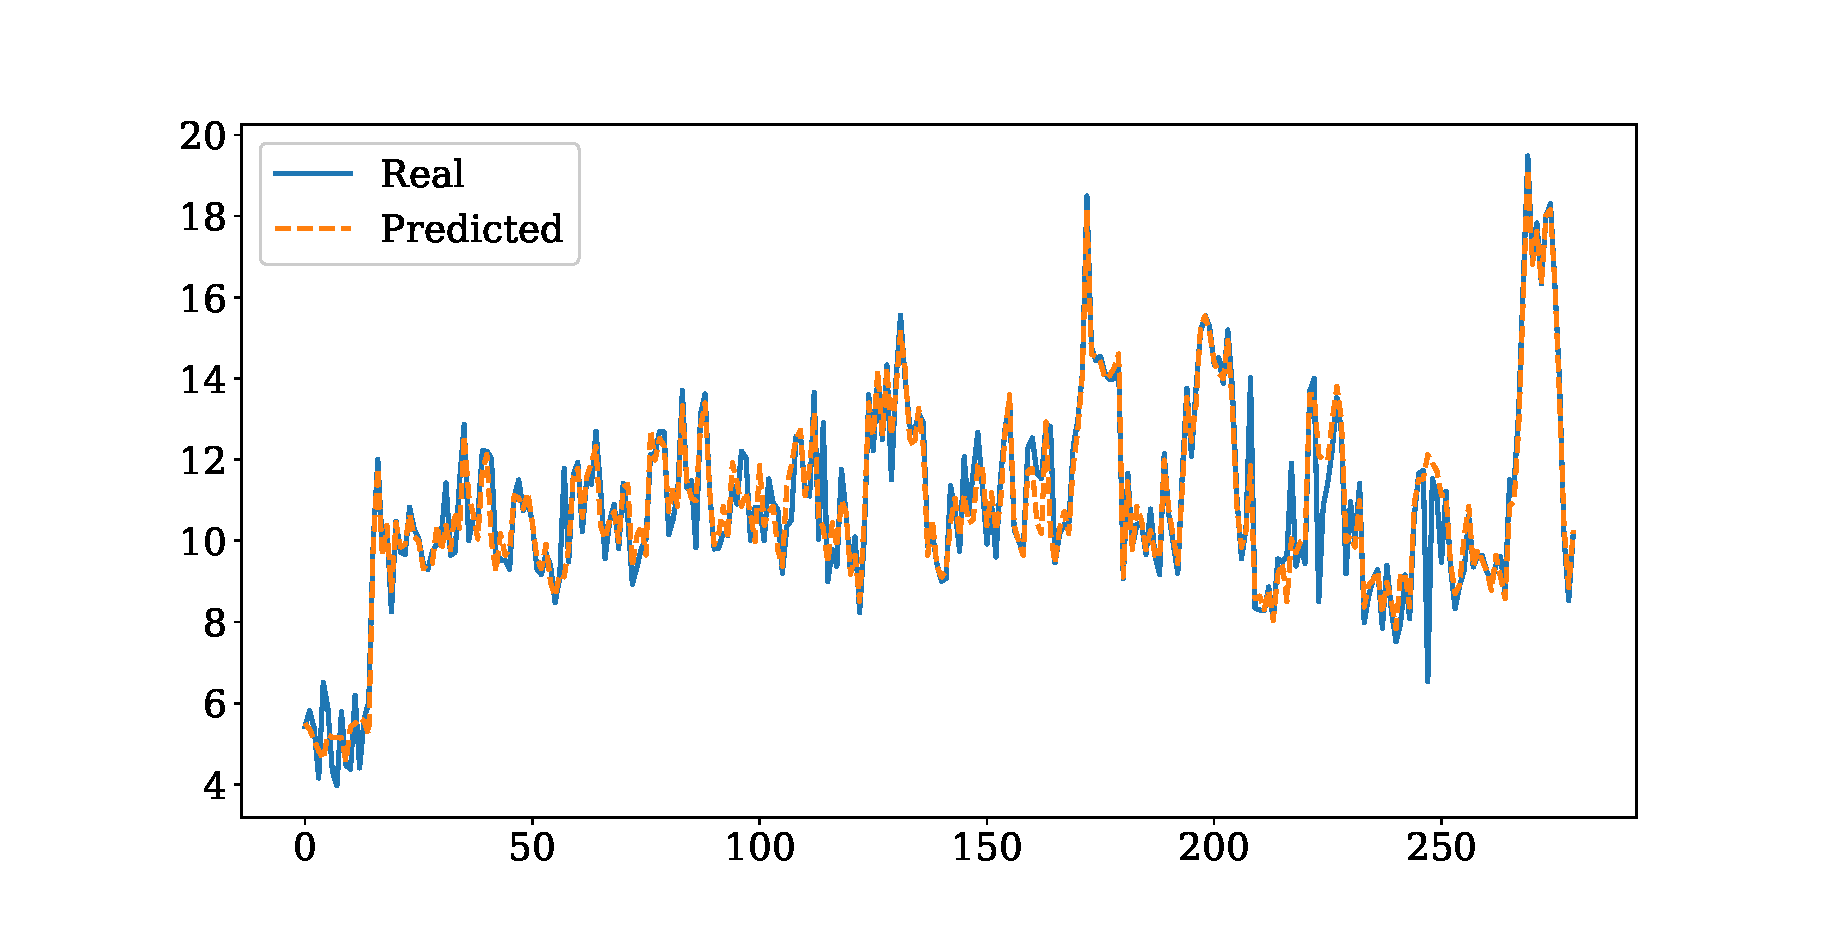
\includegraphics[width=\textwidth]{NonIdealRecovery.eps}
	\caption{Prediction reconstruction in case of inaccurate correlation matrix $\mathbf{\Sigma}$ prediction. In addition to the prediction error caused by noise in the correlation matrix a new type of error is added. When selecting a set, it is possible that the diameter is minimised not at the right set, as this is only a necessary condition, but not a sufficient one.}
	\label{fig:fig4}
\end{figure}

\section{Experiment}

In this section we test the algorithm when the pairwise correlation matrix prediction from the previous section is inaccurate. Experiments are performed on synthetic data as well as on Electricity Transformer Temperature \cite{haoyietal-informer-2021} data. Different values of $K$ are tested, as well as different added noise to the true matrix values.

\paragraph{Synthetic data.} The table below shows the error values after reconstruction the time series values under different conditions. Generated data consisting of a combination of noisy sines and cosines is used.

\begin{table}[!h]
\def\arraystretch{2.3}
\begin{center}
\caption{Loss on synthetic data. As expected, the error is less on bigger $K$ value. See \ref{fig:fig5} for the example of reconstruction with $K=10$ and noise $\mathcal{N}(0, 0.05)$.}
\begin{tabular}{|l||l||*{3}{c|}}\hline
	{Noise}
	&\makebox[3em]{Metric}&\makebox[3em]{$K=2$}&\makebox[3em]{$K=4$}&\makebox[3em]{$K=10$}\\\hline
	$\mathcal{N}(0, 0.01)$&\makecell{ MAE: \\ MSE: } &\makecell{ 0.070 \\ 0.010 }&\makecell{ 0.052 \\ 0.005 }&\makecell{ 0.040 \\ 0.002 }\\\hline
	$\mathcal{N}(0, 0.05)$&\makecell{ MAE: \\ MSE: } &\makecell{ 0.316 \\ 0.295 }&\makecell{ 0.176 \\ 0.060 }&\makecell{ 0.116 \\ 0.025 }\\\hline
	$\mathcal{N}(0, 0.1)$& \makecell{ MAE: \\ MSE: } &\makecell{ 0.530 \\ 0.635 }&\makecell{ 0.398 \\ 0.348 }&\makecell{ 0.230 \\ 0.111 }\\\hline
\end{tabular}
\end{center}
\end{table}


\begin{figure}[!htbp]
	\centering
	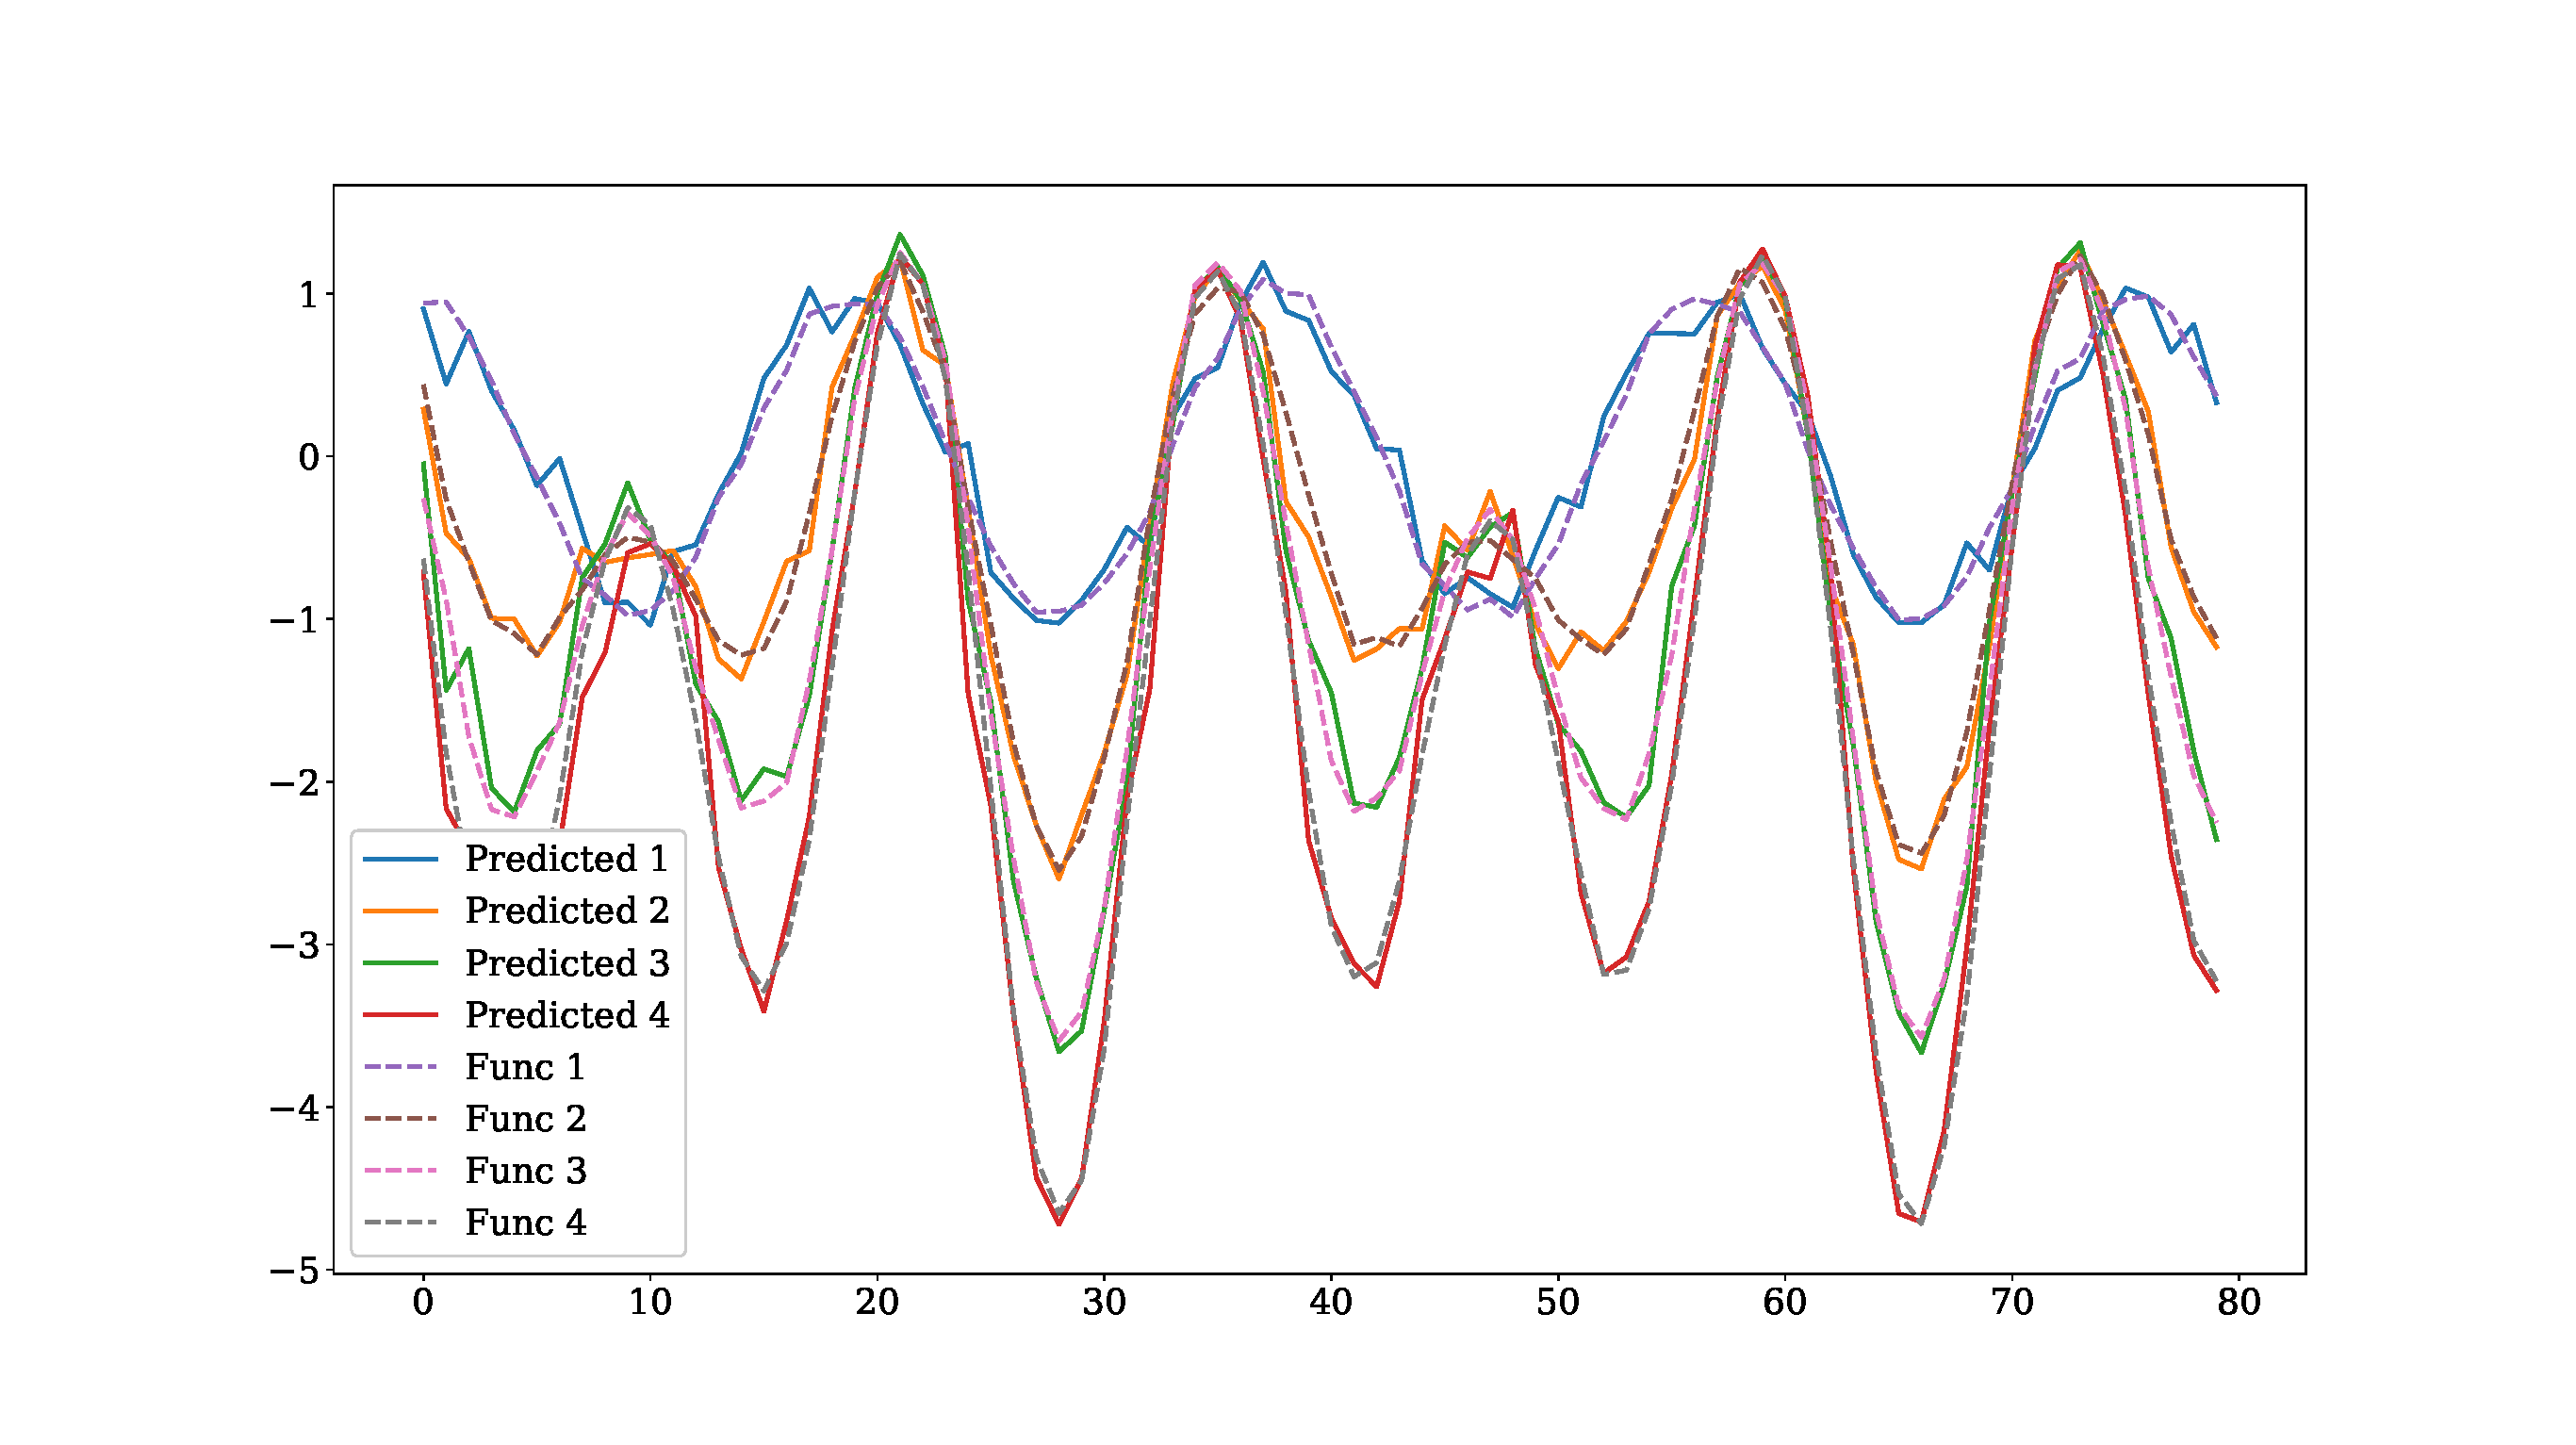
\includegraphics[width=\textwidth]{synthetic_time_series_K10N005.eps}
	\caption{Synthetic data reconstruction plot at $K=10$, Additional noise $\mathcal{N}(0, 0.05)$. \textbf{MAE: 0.116, MSE: 0.025}}
	\label{fig:fig5}
\end{figure}

\paragraph{Electricity Transformer Temperature}\

The following is a similar table for the Electricity Transformer Temperature dataset.

\begin{figure}[!htbp]
	\centering
	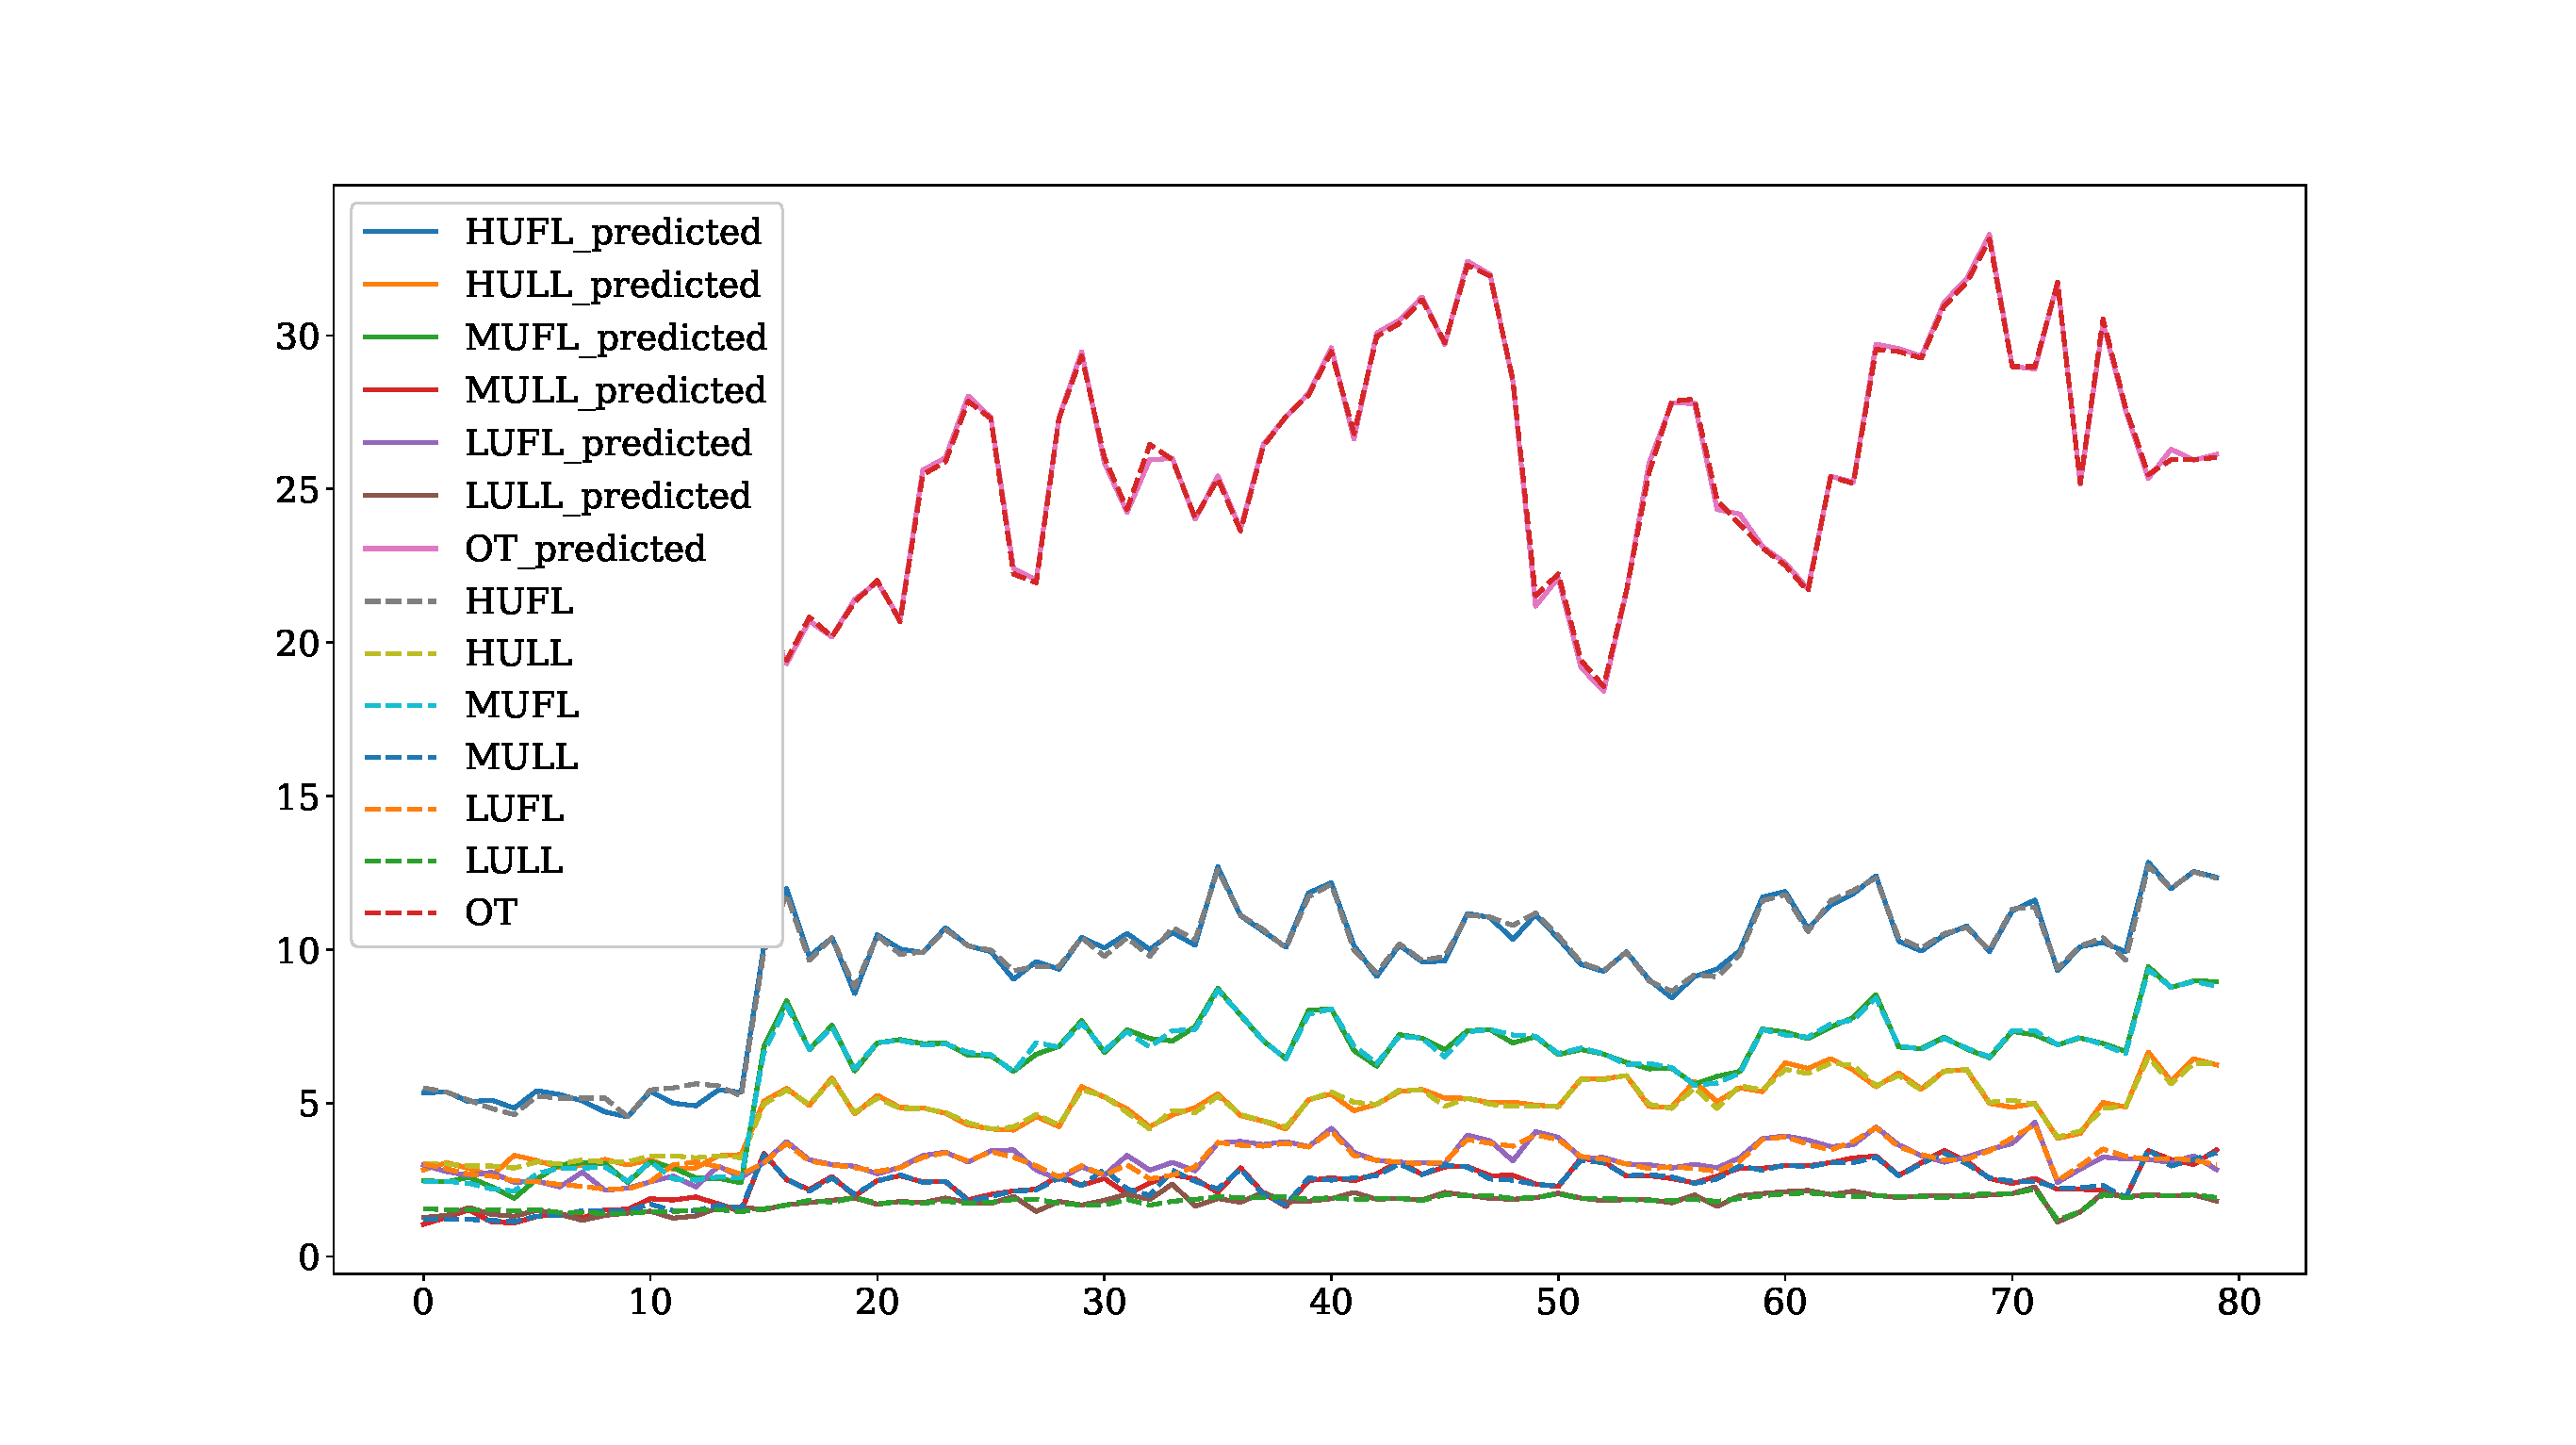
\includegraphics[width=\textwidth]{ETT_time_series_K10N005.eps}
	\caption{ETTh1 data reconstruction plot at $K=10$, Additional Noise $\mathcal{N}(0, 0.05)$. \textbf{MAE: 0.096, MSE: 0.019}}
	\label{fig:fig6}
\end{figure}

\begin{table}[!h]
\def\arraystretch{2.3}
\begin{center}
\caption{Loss on ETTh1 data. The same dependence of the error on the value of $K$ as on the synthetic data can be seen. See \ref{fig:fig6} for the example of reconstruction with $K=10$ and noise $\mathcal{N}(0, 0.05)$.}
\begin{tabular}{|l||l||*{3}{c|}}\hline
	{Noise}
	&\makebox[3em]{Metric}&\makebox[3em]{$K=2$}&\makebox[3em]{$K=4$}&\makebox[3em]{$K=10$}\\\hline
	$\mathcal{N}(0, 0.01)$&\makecell{ MAE: \\ MSE: } &\makecell{ 0.071 \\ 0.030 }&\makecell{ 0.047 \\ 0.004 }&\makecell{ 0.038 \\ 0.003 }\\\hline
	$\mathcal{N}(0, 0.05)$&\makecell{ MAE: \\ MSE: } &\makecell{ 0.240 \\ 0.198 }&\makecell{ 0.153 \\ 0.053 }&\makecell{ 0.096 \\ 0.019 }\\\hline
	$\mathcal{N}(0, 0.1)$& \makecell{ MAE: \\ MSE: } &\makecell{ 0.466 \\ 0.719 }&\makecell{ 0.306 \\ 0.281 }&\makecell{ 0.217 \\ 0.148 }\\\hline
\end{tabular}
\end{center}
\end{table}


In all cases, using more different values of $T$ predictably gave the highest accuracy. However, for $K > 15$ the algorithm becomes too computationally complex due to the exponential dependence on $K$.

\section{Conclusion}
The paper investigates an approach to time series prediction using a pairwise correlation matrix between series. It is shown that the use of only one matrix leads to the existence of a pair of possible values of the series at the next moment of time. An explicit formula for computing one answer through the other is derived, which allows the problem to be solved using non-convex optimisation. Moreover, an explicit form of the pair of answers via the singular value decomposition of the pairwise correlation matrix is derived. Two algorithms are proposed to identify the desired answer from a pair of possible answers. The first one relies on the exact prediction of the pairwise correlation matrix. The second one admits the presence of an error in the prediction, but it is more computationally demanding.

The future development of the study is to find a way to predict the pairwise correlation matrix with high accuracy. Using basic regression models give insufficiently accurate results. In such a prediction, errors are often made by incorrectly selecting the set of answers from Algorithm 2. 

Also, the side of development can be the estimation of the error radius when reconstructing the value of time series from the matrix of pair correlations. In addition, it makes sense to consider other functions of pairwise distance as a metric.


\printbibliography

\end{document}